\documentclass[tc, manuscript]{copernicus}

\usepackage{booktabs}
\usepackage{multirow}
\usepackage{siunitx} %for SI units

\begin{document}

\title{Fountain scheduling strategies to improve water use efficiency of artificial
ice reservoirs (Icestupas)}

\def\Authors{Suryanarayanan Balasubramanian\,$^{1,2}$, Martin Hoelzle\,$^{1}$Roger Waser\,$^{3}$,Martin Von Burg\,$^{3}$,}
\def\Address{$^{1}$University of Fribourg, Department of Geosciences, Fribourg, Switzerland $^{2}$University of
Applied Sciences and Arts, Luzern, Switzerland} \def\corrAuthor{Suryanarayanan Balasubramanian}
\Author[1,2]{Suryanarayanan}{Balasubramanian}
\Author[1]{Martin}{Hoelzle}
\Author[3]{Roger}{Waser}
\Author[3]{Martin}{Von Burg}
\affil[1]{University of Fribourg, Department of Geosciences, Fribourg, Switzerland}
\affil[2]{Himalayan Institute of Alternatives, Ladakh, India}
\affil[3]{University of Applied Sciences and Arts, Luzern, Switzerland}

\correspondence{suryanarayanan.balasubramanian@unifr.ch}

\runningtitle{Scheduling AIR fountains}

\runningauthor{S. Balasubramanian}

\firstpage{1}

\maketitle

\begin{abstract}

  Artificial Ice Reservoir (AIR), often also called - Ice Stupa - are a climate adaptation strategy developed in the Indian Himalayas (Ladakh). With this technology, otherwise unused stream or lake water is stored in large ice towers in winter. The melt water that is then available in spring is used for irrigation in agriculture when the melt water from glaciers is still not sufficient. Recent studies have shown that during construction of traditional AIRs over 75 \% of the water sprayed was lost. Therefore, fountain wastewater production have to be reduced to improve water use efficiency. Improved fountain scheduling was realized using an automation system that computes recommended discharge rates using real-time weather inputs and location metadata. During the winter of 2021-22, a traditional and an automated AIR were built in Guttannen, Canton of Berne, Switzerland with the main aim of comparing and quantifying the benefits of using such automation systems.
  The scheduled fountain produced similar ice volumes while consuming 87 \% lesser water than the unscheduled fountain. Overall, these results show that scheduled fountains can increase the water use efficiency without compromising on meltwater production.

\end{abstract}

\introduction

In some arid mountain regions the lack of glacier meltwater is the main constraint on agricultural production.
As the area irrigated is often governed by the limited availability of water or labour to carry water, there is
much interest at the village level in adopting water storage techniques. One such technique that has gained many
users is called artificial ice reservoirs (AIRs) or icestupas. These AIRs are traditionally constructed by
diverting glacial streams into fountain spray systems via embankments and pipelines. However, traditional
construction strategies require significant maintenance and produce high water losses. Improvement of these
construction strategies, therefore, will allow the farmers to cultivate larger areas or to devote more time to
other activities. 

Several AIR construction efforts have been abandoned despite having favourable weather conditions. This is
because colder weather conditions  not just build bigger AIRs but also increase maintenance and pipeline damage
by also freezing water inside the pipeline. In order to circumvent these issues, AIR constructors often maintain
the maximum possible flow in the pipeline even during time periods when temperature conditions are far from
ideal. This reduces the risk of pipeline freezing events but at the expense of water use efficiency. However,
AIR constructors also increase the fountain periodically which lowers the discharge rate and thereby increases
the risk of pipeline freezing events. Hence, traditional AIR constructions often come to a halt in the middle of
winter when increases in height and fluctuations of weather inevitabily leads to a pipeline freezing event.

An optimum construction strategy, therefore, should prevent pipeline freezing events while maintaining high
water use efficiency. Typical solutions to prevent pipeline freezing events are to bury or drain the pipeline.
Burying the pipeline at a sufficient depth can reduce the influence of atmospheric conditions on the pipeline
water temperature. Even though this method is ideal, it can quickly get expensive depending on the length of the
pipeline and the frost depth. Therefore, such an effort is warranted only in the case of a permanent
construction location. Comparatively, draining the pipeline is a much cheaper strategy. Moreover, it can be
combined with fountain scheduling methods to achieve reduced watering volumes for AIR construction systems.

Proper fountain scheduling requires answers to two questions: 
(a) When should the water be turned on and off?
(b) How much water should be sprayed? 

For answering these questions, knowledge of surface freezing rates is important . Surface freezing rates can be
calculated by means of the full energy balance model developed in
\cite{balasubramanianInfluenceMeteorologicalConditions2022}. But this model needs to be forced with weather data
to recommend fountain scheduling strategies. Historical weather data or real-time weather data could be used to
force the model. To accomodate for the limited quantity of data available in any new location, we further
approximate the model by including two kinds of assumptions that are considerate for the limited water
availability or the favourable weather windows respectively.

However, maually adjusting the fountain discharge rate is unrealistic . Firstly, constant adjustments of
discharge rates in response to the significant diurnal and seasonal variations of the freezing rates is
impractical. Secondly, frequent pipeline water drainage required to prevent freezing events during critical weather
windows is unfeasible. Therefore, operation of scheduled fountains via automation systems is preferred.

The main interest in using model results is to simulate fountain schedules relative to various constrains in
favourable weather windows and water availability. The fountain scheduling strategies are evaluated from the
relative water use efficiency and maximum ice volume produced during the construction period. The specific
objectives of this paper include the presentation of the automation system and examples of its application to
the computation of fountain scheduling strategies.

\section{Study site and data}

The Guttannen site (46.66 $\degree$N, 8.29 $\degree$E) is situated in the Berne region, Switzerland and has an altitude of 1047 $m$ a.s.l. In the winter (Oct-Apr), mean daily minimum and maximum air temperatures vary between -13 and 15 $\degree C$. Clear skies are rare, averaging around 7 days during winter. Daily winter precipitation can sometimes be as high as 100 $mm$. These values are based on 30 years of hourly weather model simulations \citep{guttannen}. Two AIRs were constructed by the Guttannen Bewegt Association, the University of Fribourg and the Lucerne University of Applied Sciences and Arts during the winters of 2021-22 using a traditional and an automated construction strategy.

\begin{figure}[t]
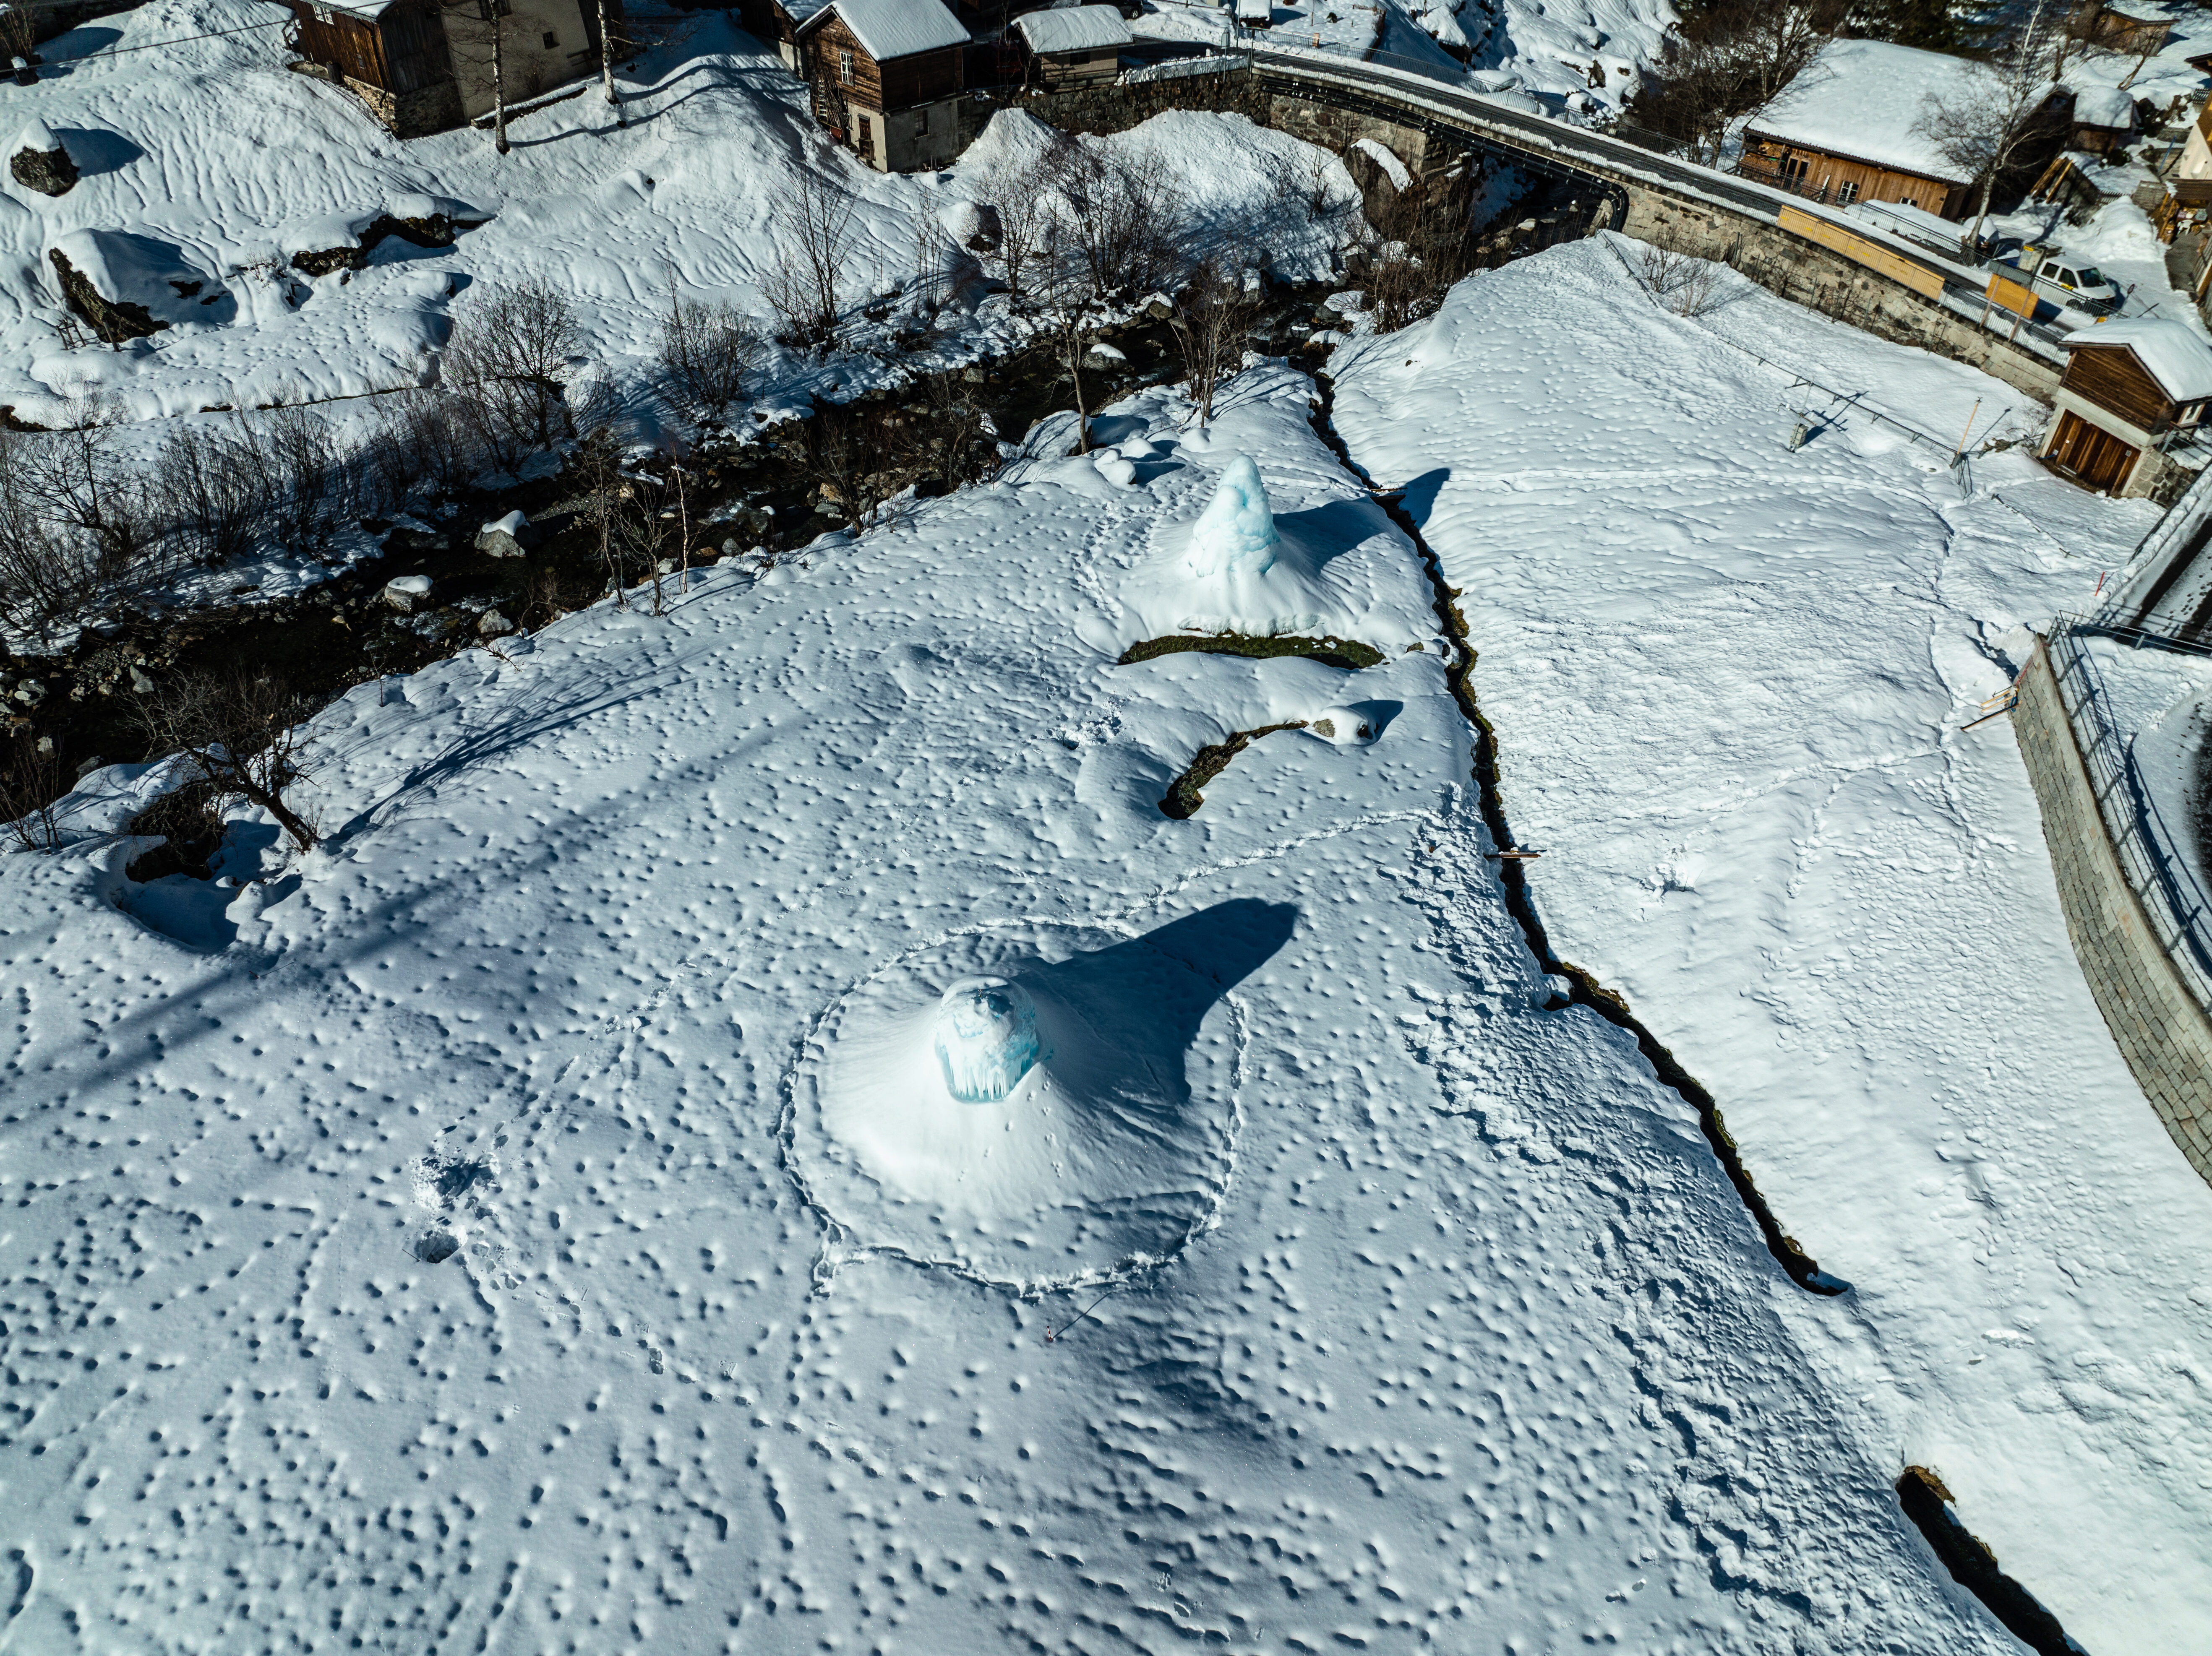
\includegraphics[width=8.3cm]{Figures/2AIRs.jpg}
\caption{Automated and traditional AIRs  at Guttannen on February 6, 2022. Picture credits: Daniel Bürki}
\label{fig:2AIR} 
\end{figure}

In order to compare both the construction strategies, the automated and the traditional AIRs were constructed
adjacent to each other as shown in Fig. \ref{fig:2AIR}. This ensured both AIRs shared the same water source
and similar weather conditions. In addition, a webcam guaranteed a continuous survey of the automated AIR.   

In the traditional strategy, tree branches were laid covering the fountain pipe to initiate and speed up of generating a fast ice cone formation process. The fountain discharge was maintained at maximum and its height was increased from 3 to 6\,$m$ during the construction period.

In the automated strategy, only the fountain pipe was placed before the water spray started. A programmed automation system controlled the fountain discharge rate during the whole winter season using real time weather input and several control parameters, which could be tested and controlled via a data logger user interface. 

\subsection{Meteorological data}

Air temperature, relative humidity, wind speed, pressure, longwave, shortwave direct and diffuse radiation are
required to calculate the surface energy balance of an AIR (see Fig. \ref{fig:aws}). The construction period
starts when the fountain was first switched on and ends when the fountain was last switched off. These two dates
are denoted as start and fountain off dates henceforth.

\begin{figure*}[t]
\includegraphics[width=12cm]{Figures/data.png}
\caption{Temperature, precipitation and discharge measurements at the Guttannen construction site}
\label{fig:aws} 
\end{figure*}

The weather data source was an automatic weather station (AWS) located around 20 m away as shown in Fig. \ref{fig:2AIR}. Less than 0.4 \% of the data was found to be corrupted and these were filled by linear interpolation. 
We define the fountain used through four attributes by the spray radius, the discharge rate, the pipe height and the water temperature.

\subsection{Fountain observations}

 The spray radius $r_F$ was estimated from the mean AIR circumference measured in the drone surveys during the fountain runtime. The discharge rate of the scheduled fountain was measured by the automation system. The discharge of the unscheduled fountain was using the maximum discharge rate recorded by the automation system. This was because the unscheduled fountain has been spraying the maximum discharge rate during the full construction period. However,
the discharge rate was reduced by half whenever a new pipe of 1 m length was installed to increase the fountain height. The same reduction in magnitude was also well observed for the scheduled fountain discharge rate. Therefore, we determine the discharge of the traditional fountain by using the measurements of the discharge rate for the automated fountain. A new fountain design was used for the automated strategy since the traditional fountain design was unable to function in the whole range of discharge rates suggested by the automation system.

\subsection{Drone surveys}

Several photogrammetric surveys were conducted on the traditional and the automated AIRs. The details of these surveys and the methodology used to produce the corresponding outputs are explained in the Appendix. The digital elevation models (DEMs) generated from the obtained imagery were analysed to document the spray radius, the surface area and the volume of the ice structures. The number of drone surveys conducted for the traditional and the automated AIRs were 6 and 3, respectively (see Table). The last drone flight was used to set the dome volume for the traditional AIR. The dome volume for the automated AIR represented the snow volume found before the fountain was switched on. The remaining surveys were used for model validation.

\begin{table}
	\centering
	\caption{ Summary of the drone surveys}
	\label{tab:uav}
	\begin{tabular}{@{}|llllll|@{}}
		\toprule
		\textbf{}              & \textbf{No.} & \textbf{Date} & \textbf{Volume} & \textbf{Radius} & \textbf{Surface Area} \\ \midrule
		\multicolumn{1}{|l|}{\multirow{6}{*}{\rotatebox[origin=c]{90}{Traditional}}}
		                       & 1            & Dec 23, 2021  & 17 $m^{3}$     & 2.9 $m$
		                       & 47 $m^{2}$                                                                      \\
		\multicolumn{1}{|l|}{} & 2            & Jan 3, 2022  & 22 $m^{3}$     & 3.4 $m$
		                       & 61 $m^{2}$                                                                      \\
		\multicolumn{1}{|l|}{} & 3            & Jan 22, 2022   & 626 $m^{3}$     & 4 $m$
		                       & 79 $m^{2}$                                                                      \\
		\multicolumn{1}{|l|}{} & 4            & Feb 6, 2022  & 44 $m^{3}$     & 4.2 $m$
		                       & 86 $m^{2}$                                                                      \\
		\multicolumn{1}{|l|}{} & 5            & Feb 12, 2022  & 62 $m^{3}$     & 4.2 $m$
		                       & 108 $m^{2}$                                                                      \\
		\multicolumn{1}{|l|}{} & 6            & & $m^{3}$     & $m$
		                       & $m^{2}$
		\\\midrule
		\multicolumn{1}{|l|}{\multirow{3}{*}{\rotatebox[origin=c]{90}{Automatic}}}
		                       & 1            & Dec 23, 2021  & 22 $m^{3}$      & 3.7 $m$
		                       & 57 $m^{2}$                                                                       \\
		\multicolumn{1}{|l|}{} & 2            & Jan 3, 2022   & 30 $m^{3}$      & 3.9 $m$
		                       & 66 $m^{2}$                                                                       \\
		\multicolumn{1}{|l|}{} & 3            &               &    $m^{3}$      &     $m$
		                       &    $m^{2}$                                                                       \\
		\bottomrule
	\end{tabular}

\end{table}

\section{Methods}

\subsection{Automation system}

\subsubsection{Automation hardware}

The automation system implements fountain scheduling strategies for the twin objectives of ice volume (ICV) and water use efficiency (WUE). The ICV objective is suitable at locations with sufficient water volumes to
freeze during the construction period. The WUE objective is suitable at locations with favourable weather conditions constrained by available water supply. For the ICV objective, the model assumptions overestimate the freezing rate whereas for the WUE objective the model assumptions underestimate the freezing rate. 

The automation hardware consists of an AWS, flowmeter, control valve, drain valves, air valves, fountain, pipeline and a logger. The logger feeds the AWS data to the automation software and informs the recommended discharge rate to the flowmeter. The flowmeter adjusts the control valve to match the
recommendation. However, the recommended discharge rate is ignored if any of the termination criterion are valid. The termination criterion prevent water loss and pipeline freezing events. In case a termination criteria is valid, the drain and air valves empty the water in the pipeline.

\subsubsection{Automation software}

Any construction location can either be constrained by the available water supply or the duration of subzero
weather windows for fountain operation. If the respective location has limited water supply then the fountain
scheduling strategy should be optimised for high water use efficiency (WUE). But if the location is limited by
the time period when the fountain can function then the scheduling strategy should be optimised for high ice
volumes (ICV).

We introduce two kinds of approximations in the automation software that optimise for the ICV and WUE objective
respectively. We approximate the expected (a) AIR shape using its slope parameter, (b) AIR surface properties
using its surface albedo and (c) weather conditions using the cloudiness parameter. The assumptions are
described in the Appendix and summarised in Table \ref{tab:assumptions}. 

We assume the surface temperature is always at melting point and ignore the contribution of fountain heat
flux and ground heat flux to the energy balance to estimate both the scheduling strategies. The consequences of
these assumptions in the determination of all the energy balance terms are discussed in the Appendix.

\begin{table}[]
\centering
\caption{Assumptions introduced to simplify the model.}
\label{tab:assumptions}
\begin{tabular}{@{}lllll@{}}
\toprule
\textbf{Estimation of} & \textbf{Symbol} & \textbf{ICV Assumptions} & \textbf{WUE Assumptions} & \\ \midrule
\multicolumn{1}{|l}{AIR slope}        & $s_{cone}$ & $ 1 $ & $0$ & \multicolumn{1}{l|}{} \\ \midrule
\multicolumn{1}{|l}{Albedo} & $\alpha$ & $\alpha_{snow}$ & $\alpha_{ice}$ & \multicolumn{1}{l|}{} \\\midrule 
\multicolumn{1}{|l}{Cloudiness}  & $cld$ & $0$ & $1$ & \multicolumn{1}{l|}{} \\ \bottomrule
\end{tabular}
\end{table}

Equation \ref{eqn:auto} is implemented in the automation system through a user interface that enables input of
the spray radius, altitude, latitude and longitude of the construction location. Once switched on, the
automation system regulates the fountain discharge rate based on the recommended discharge rate. However,
certain termination criterias override the discharge rate recommendation to prevent water loss and pipeline
freezing events, namely: 

\begin{itemize}

\item Loss of water droplets due to high wind speed are avoided by introducing a wind speed limit 

\item Pipeline freezing events due to very cold conditions are avoided by setting a minimum temperature limit 

\item Pipeline damage is avoided by draining the pipeline upon a pipeline freezing event detection. Pipeline freezing events are assumed if $Q_F = 0$ for at least 20 seconds.

\item Water loss is avoided by detection of pipeline leakage/damage. Pipeline leakage is assumed if $Q_F > Q_{leak}$. 

\item Pipeline freezing events are prevented by ignoring low discharge rate recommendations  

\end{itemize}

\subsection{Calibration}
We retain the default values of all parameters used in \cite{balasubramanianInfluenceMeteorologicalConditions2022} for our analysis.  

In addition, two model variables, fountain water temperature ($T_F$) and AIR density ($\rho_{AIR}$) are parametrised. Both variables were assumed to be constant in the previous versions of the model. With the extended measurement dataset of CH22 AIR, we estimate the water temperature variable by assuming it is equal to our ground temperature measurements but only when the air temperature was not subzero. Under subzero conditions, the water droplets are likely to cool to 0 C during their flight time. Therefore, the fountain water temperature was instead determined as follows:

\begin{equation}
	T_{F} = \left\{ \begin{array}{ll}
		0 & \textit{ if } T_{temp} < 0 \\
		T_{G} & \textit{ otherwise}
	\end{array} \right.
\end{equation}

where $T_{G}$ is the measured ground temperature.

The snowfall mass input of CH22 AIR was comparable to the mass input via the fountain discharge. Therefore, we could no longer assume that the AIR density was equal to ice density. We instead parameterised AIR density $\rho_{AIR}$ as follows:

\begin{equation}
  \rho_{AIR} = \frac{M_{F} + M_{dep} + M_{ppt}}{(M_{F} + M_{dep})/\rho_{ice} + M_{ppt}/\rho_{snow}}
\end{equation}

where $M_F$ is the cumulative mass of the fountain discharge; $M_{ppt}$ is the cumulative precipitation; $M_{dep}$ is the cumulative accumulation through water vapour deposition; $\rho_{ice}$ is the ice density (917 $kg\,m^{-3}$) and $\rho_{snow}$ is the density of wet snow (300 $kg\,m^{-3}$) taken from
\cite{cuffeyPhysicsGlaciers2010} .

\subsection{Validation}
We performed the validation of the model on the traditional and automated AIRs by evaluating the root mean
squared error (RMSE) between ice volume estimates and measurements . Even though the number of drone flights
were identical for both AIRs, fewer successful volume observations were possible for the automated AIR as shown
in Table \ref{tab:uav}. This was because the DEMs generated for the automated AIR could not georeference the
automated AIR's snow covered surface. Since the traditional AIR was steeper, its surface revealed ice patches
that could be georeferenced. Root mean squared error (RMSE) served as the evaluation metric in both the cases.

The performance of the ICV and WUE versions of the physical model was assessed by comparing correlation of its
discharge rate estimates with the validated freezing rate of the calibrated physical model.

\section{Results}

\subsection{Energy balance model validation}
The physical model achieved an RMSE of $4 \degree C$ with the AIR mean temperature measurements of the automated AIR and an RMSE of $m^3$ with the ice volume measurements of the traditional AIR. The estimated and measured AIR
mean temperatures and ice volumes are shown in Fig. \ref{fig:validation}
 
\begin{figure*}[t] 
  \includegraphics[width=12cm]{Figures/validation.png} 
  \caption{Ice volume validation of the scheduled and unscheduled fountain construction strategies.} 
\label{fig:validation} 
\end{figure*}

\subsection{Scheduled discharge rate estimation}

We found that the simplified energy balance model estimated the freezing rate of the unscheduled fountain with a correlation higher than 0.5 and RMSE less than 1 $l/min$ for both the ICV and WUE objectives. The ICV scheduled fountain overestimated the freezing rate 90 \% of the construction duration whereas the WUE
scheduled fountain underestimated the freezing rate 80 \% of the construction duration as shown in Fig.
\ref{fig:freezing_rate}.

% \begin{figure*}[t]
% \includegraphics[width=12cm]{Figures/freezing_rate_corr.png}
% \caption{Scheduled discharge rate estimates of the simplified energy balance model with the WUE and ICV
% assumptions compared with the validated freezing rate of the full energy balance model.}
% \label{fig:freezing_rate}
% \end{figure*}

\subsection{Comparison of AIR construction strategies}

Table \ref{tab:mb} shows how the different fountain scheduling strategies influence the mass
and energy balance of the respective AIR. As expected, unscheduled fountains produce an order of magnitude
increase in the fountain discharge input and fountain wastewater output. 

To understand how the different scheduling strategies influence the rest of the mass balance output, we discuss
the influence of fountain discharge on the surface mass and energy balance. During fountain spray, the AIR
surface is affected in the following three ways, namely, (a) its albedo dampens to ice albedo, (b) its
temperature warms to 0 C and (c) it absorbs the heat energy of the fountain water droplets. These three
processes are the cause of the difference in the mass and energy balance distribution shown in  Table
\ref{tab:mb}. The temporal variation of the magnitude of all these three processes are shown in Fig. In general,
all the three processes affect the mass and energy balance of the traditional AIR much more than the Automated
AIR since its fountain duration was ? times higher. 

To understand the overall impact of the radiation fluxes (longwave and shortwave) and the turbulent fluxes
(sensible and latent) on the freezing and melting energies, we sum their respective energy turnover by taking
into account the sign of their mean energy during the study period (see Table \ref{tab:mb}). A negative sign
indicates that the corresponding energy flux increased/decreased the freezing/melting energy respectively.  The
radiation fluxes contributed -25 \% and -17 \% to the freezing energies for the traditional and automated AIR,
respectively.  Similarly, the turbulent fluxes contribute -13 \% and -9 \% to the freezing energies for the
traditional and automated AIR, respectively. The fountain water and ground heat flux contribute 10 \% and 5 \%
to the melting energies for the traditional and automated AIR, respectively. 

Even though the distribution of the radiation fluxes is similar, there is a considerable difference in the
magnitude of these fluxes between the AIRs. In particular, the shortwave and longwave radiation is higher and
lower for the traditional AIR due to the effect of processes (a) and (b) respectively. Similarly, the reduced
contribution of sensible heat in the turbulent fluxes of the traditional AIR is a consequence of process (b).
The fountain water heat flux is enhanced whereas the ground heat flux is dampened by process (c).


\begin{table}
	\centering
	\caption{ Summary of the mass balance and AIR characteristics estimated at the end of the respective
  simulation duration for the automated and the traditional AIRs}
	\label{tab:mb}
	\begin{tabular}{@{}|llllll|@{}}
		\toprule
		\textbf{}              & \textbf{Name}                   & \textbf{Symbol} & \textbf{Traditional} & \textbf{Automated} &
		\textbf{Units}                                                                                                       \\ \midrule
		\multicolumn{1}{|l|}{\multirow{3}{*}{\rotatebox[origin=c]{90}{Input}}}
		                       & Fountain discharge              & $M_F$           & \num{7.3e5}   & \num{7.5e4}     & $kg$  \\
		\multicolumn{1}{|l|}{} & Snowfall                        & $M_{ppt}$       & \num{1.3e4}   & \num{2.2e4}   & $kg$  \\
		\multicolumn{1}{|l|}{} & Deposition                      & $M_{dep}$       & \num{2.3e2}   & \num{8.9e2}     & $kg$  \\ \midrule
		\multicolumn{1}{|l|}{\multirow{4}{*}{\rotatebox[origin=c]{90}{Output}}}
		                       & Meltwater                       & $M_{water}$     & \num{2.0e4} & \num{1.2e4}   & $kg$  \\
		\multicolumn{1}{|l|}{} & Ice                             & $M_{ice}$       & \num{2.2e4} & \num{3.0e4}    & $kg$  \\
		\multicolumn{1}{|l|}{} & Sublimation                     & $M_{sub}$       & \num{1.5e3} & \num{1.2e3}     & $kg$  \\
		\multicolumn{1}{|l|}{} & Fountain wastewater             & $M_{waste}$     & \num{7.0e5} & \num{6.5e4}     & $kg$  \\ \midrule
		\multicolumn{1}{|l|}{\multirow{7}{*}{\rotatebox[origin=c]{90}{Energy Balance}}}

                           & Shortwave radiation             &  $q_{SW}$       & $25$  & $26$ & \% \\
		\multicolumn{1}{|l|}{} & Longwave radiation              &  $q_{LW}$       & $-45$  & $-43$ & \% \\
		\multicolumn{1}{|l|}{} & Sensible heat                   &  $q_{S}$        & $4$   & $8$ & \% \\
		\multicolumn{1}{|l|}{} & Latent heat                     &  $q_{L}$        & $-17$  & $-17$ & \% \\
		\multicolumn{1}{|l|}{} & Fountain water heat             &  $q_{F}$        & $9$  & $1$     & \% \\
		\multicolumn{1}{|l|}{} & Ground heat                     &  $q_{G}$        & $1$   & $4$     & \% \\\midrule
		\multicolumn{1}{|l|}{\multirow{2}{*}{\rotatebox[origin=c]{90}{AIR}}}

		                       & Maximum Ice Volume              &                 & 47            & 67            & $m^{3}$ \\
		\multicolumn{1}{|l|}{} & Water Use Efficiency            &                 & 5             & 38            & \% \\
		\multicolumn{1}{|l|}{} & Surface Area                    &  $A_{cone}$     & $56\pm 5$  & $79 \pm 4$     &$m^{2}$ \\\midrule
	\end{tabular}
\end{table}

\section{Discussion}

\subsection{Simulations of scheduled fountains}

We evaluate the benefits of the automated construction strategies by comparing them with the traditional construction strategies used in the IN21 and CH21 locations presented in
\cite{balasubramanianInfluenceMeteorologicalConditions2022}. The difference in water use efficiency and maximum ice volumes expected between unscheduled and scheduled fountains in the three locations are presented in Fig.
\ref{fig:wue}.

\begin{figure*}[t]
\includegraphics[width=12cm]{Figures/wue.png}
\caption{The maximum ice volume and water use efficiency estimated for the different locations and construction
strategies used}
\label{fig:wue}
\end{figure*}


\conclusions
In this paper, an automated AIR construction strategy is presented and compared with a traditional strategy
using data collected in Guttannen, Switzerland.

The main purpose of this study was to test the idea that scheduled AIR fountains could lead to a significant
improvement in water use efficiency and ice volumes. A simplified energy balance model compatible with the
limited data availability of a new location was used to produce recommended discharge rate. Nevertheless, this
model was able to capture more than 65 \% of the freezing rate variations produced by the full energy balance
model.

The automation system allows the easy handling of fountain scheduling implementation. The possibility for
changing the location and fountain metadata directly in the user interface allows tailoring the fountain
discharge rate according to the location's water supply and weather conditions. Furthermore, this construction
strategy reduces the occurence of pipeline freezing events as it drains the pipeline whenever critical weather
windows are detected.

Nevertheless, the real world application of this method is challenging. It is clear that if improvements are to
be achieved, future research must be devoted to modelling the impact of fountain design on the spray radius.

\appendix

\section{Simplified energy balance model}

We approximate the energy balance at the surface of an AIR by a one-dimensional description of energy fluxes as
used in \cite{balasubramanianInfluenceMeteorologicalConditions2022}. The ice volume evolution of the AIR can be
represented as: 

\begin{equation}
  \frac{\Delta V_{ice}}{\Delta t}  =  \frac{\Delta j_{cone}}{ \Delta t} \cdot A_{cone}
	\label{eqn:freeze}
\end{equation}

where $\frac{\Delta j_{cone}}{\Delta t}$ is the thickness change determined as follows:

\begin{equation}
  \frac{\Delta j_{cone}}{\Delta t}  = \frac{1}{\rho_{AIR}} \cdot (\frac{q_{SW} + q_{LW} + q_{S} + q_{F} + q_{G} -
  q_{T}}{L_F} + \frac{q_{L}}{L_V} )
	\label{eqn:freeze}
\end{equation}

Upward and downward fluxes relative to the ice surface are positive and negative, respectively. The first term
represents the surface thickness change rate due to freezing of the fountain water and melting of the ice.
$q_{SW}$ is the net shortwave radiation; $q_{LW}$ is the net longwave radiation; $q_{L}$ and $q_{S}$ are the
turbulent latent and sensible heat fluxes; $q_{F}$ is the fountain heat flux; $q_{G}$ is the ground heat flux
and $q_{T}$ is the temperature heat flux. However, we assume $q_{F}$, $q_{G}$ and $q_{T}$ to be negligible.

The data requirement was reduced by estimating the global shortwave radiation and pressure directly using the
location's coordinates and altitude through the solar radiation model described in
\citet{holmgrenPvlibPythonPython2018}. The algorithm used to estimate the clear-sky global radiation is
described in \citet{ineichenBroadbandSimplifiedVersion2008}.  

The model complexity was reduced through assumptions that optimise for the ice volume objective or the water use
efficiency objective. Assumptions are chosen based on whether they overestimate/underestimate the freezing rate.
Ice volume objective requires freezing rate to be overestimated whereas WUE objective requires freezing rate to
be underestimated. We describe these two kinds of assumptions applied on each of the energy balance components
below: 

\subsection{Surface Area $A_{cone}$ assumptions}

Since we are only interested in determination of the surface area during the accumulation period we can assume a
constant ice cone radius equal to the fountain spray radius. The surface area scales the freezing rate of the
AIR. Hence, for the ICV objective we assume the maximum possible slope of 1 for the ice cone or in other words
$h_{cone} = r_{F}$. Therefore, area is estimated as:  

\begin{equation} A_{cone} =\pi \cdot r_{F}^2 \label{eq:Area} \end{equation}

Similarly, for the WUE objective, the area of the conical AIR is approximated to the area of its circular
base.Therefore, area is estimated as:

\begin{equation} A_{cone} =\sqrt{2} \cdot \pi \cdot r_{F}^2 \label{eq:Area} \end{equation}

\subsection{Net shortwave radiation \texorpdfstring{$q_{SW}$}{Lg} assumptions}
\label{sec:SW}

The net shortwave radiation $q_{SW}$ is computed as follows:

\begin{equation} 
q_{SW} = (1- \alpha) \cdot ( SW_{direct} \cdot f_{cone} + SW_{diffuse})
\label{eqn:SW} 
\end{equation}

where $\alpha$ is the albedo value ; $SW_{direct}$ is the direct shortwave radiation; $SW_{diffuse}$ is the
diffuse shortwave radiation and $f_{cone}$ is the solar area fraction.

The diffuse and direct shortwave radiation is determined using the estimated global solar radiation as follows:

\begin{equation}
\begin{split}
  SW_{diffuse} &= cld \cdot SW_{global}\\
  SW_{direct} &= (1-cld) \cdot SW_{global}
\end{split}
\end{equation}

where $cld$ is the cloudiness factor. $cld$ is assumed to be 1 and 0 for the WUE and iceV objective
respectively.

We ignore the variations in the albedo and assume it to be equal to snow albedo and ice albedo for the iceV and
WUE objective respectively. 

The solar area fraction $f_{cone}$ of the ice structure exposed to the direct shortwave radiation depends on the
shape considered. It is computed as

\begin{equation}
		f_{cone} =\frac{(0.5 \cdot r_{cone} \cdot h_{cone}) \cdot cos \theta_{sun} +(\pi \cdot
			{(r_{cone})}^2/2) \cdot sin \theta_{sun} }{\pi \cdot r_{cone} \cdot ({(r_{cone})}^2+{(h_{cone})}^2)^{1/2}}\\
\end{equation}

For the ICV objective, since we assume the slope of the cone to be 1 $f_{cone}$ is determined
as follows:

\begin{equation}
		f_{cone} =\frac{ cos \theta_{sun} + \pi \cdot sin \theta_{sun} }{2\sqrt{2} \cdot \pi }
\end{equation}

Similarly, for the WUE objective, since we assume the slope of the cone to be negligible, we get:

\begin{equation}
		f_{cone} =\frac{ sin \theta_{sun} }{2 }
\end{equation}

\subsection{Net Longwave radiation \texorpdfstring{$q_{LW}$}{Lg} assumptions} \label{sec:LW}

We assume $T_{ice} = 0 \degree C$ in order to determine outgoing longwave radiation. Since it is challenging to
contrain the minimum ice temperature, we maintain this assumption for both our objectives. However, in order to
estimate atmospheric emissivity we again assume $cld$ to be 1 and 0 for the WUE and iceV objective respectively.

\subsection{Turbulent fluxes assumptions} \label{sec:Qs}

Turbulent fluxes estimation depend on the slope of the cone through the $\mu_{cone}$ parameter. As suggested 
by \citet{oerlemansBriefCommunicationGrowth2021}, we can estimate this parameter as follows:

\begin{equation}
  \mu_{cone} =1 + s_{cone}/2
\end{equation}

Hence, the $\mu_{cone}$ parameter takes values of 1.5 and 1 for the iceV and WUE objective respectively.  Since
turbulent fluxes impact both the freezing and the melting rates, this assumption may not favor the corresponding
objectives for certain sites.


\noappendix 

\bibliographystyle{copernicus}
\bibliography{zot_refs.bib}

\end{document}
